
\documentclass{article}
\usepackage{utf8math,ttquot,mathpartir,amsmath, amssymb, hydrocomments, mathtools,multicol,xspace}
\usepackage[margin=1in]{geometry}
\begin{document}

\abstract{Adding properties to hydroflow is important, because it
  allows us to do three things: (1) it lets us explicitly state and
  verify the requirements individual hydroflow operators have assumed
  of their inputs in order to be correct, (2) It allows us to encode
  translational goals and optimization correctness conditions, and (3) }

\section{technical todo}

\begin{itemize}
\item Type system: basic structure and derivations ✓
\item Type system: properties and their satisfaction
\item semantics: core semantic model (is it rewrite-based?)
\item Type system: axiom rewrite system
\item core language: axiom extensibility
\item proof: progress+preservation (or its equivalent in axiomatic semantics)
\item proof: axiom admissibility (via bisimulation?)
\item evaluation: example programs which satisfy the above
\item evaluation: programmability assessment
\item evaluation: extensibility assessment (new operators)
\end{itemize}

\section{syntax}

\newcommand{\closedprogram}{\textit{closed-program}\xspace}
\newcommand{\compiledcomponent}{\textit{compiled-component}\xspace}
\newcommand{\incast}{\textit{incast}\xspace}
\newcommand{\outcast}{\textit{outcast}\xspace}
\newcommand{\seqstart}{\textit{seq-start}\xspace}
\newcommand{\seqend}{\textit{seq-end}\xspace}
\newcommand{\chain}{\textit{chain}\xspace}
\newcommand{\op}{\textit{op}\xspace}
\newcommand{\opt}{τ_{\textit{op}}\xspace}
\newcommand{\N}{ℕ}
\newcommand{\fresh}{\textit{fresh}\xspace}
\newcommand{\inputs}{\textit{inputs}\xspace}
\newcommand{\outputs}{\textit{outputs}\xspace}
\newcommand{\IT}[1]{{\textit{#1}}\xspace}

\begin{figure}
  \begin{align*}
    \closedprogram &:= "declare"~ A…~"in"~ p\\
    A &∈ \textit{handoff-names}\\
    p_\IT{out} &:= [p_\IT{out}]\op ∣ A ∣ (p_\IT{out}|p_\IT{out})\\
    p_\IT{in} &:= [p_\IT{in}]\op ∣ A ∣ (p_\IT{in}|p_\IT{in})\\
    p &:= [p_\IT{in}]\op[p_\IT{out}] ∣ (p|p)
  \end{align*}
  \label{fig:syntax}
  \caption{Syntax}
\end{figure}


In figure \ref{fig:syntax}

\section{types}

\begin{figure}
  \begin{mathpar}

    {\inferrule{A : in(dₐ), A : out(dₐ),… ;A : τₐ,…  ⊢ p}
      {⊢ "declare"~A…~"in"~p}}
    
    {
      \inferrule[pivot]{\inputs(\op) = τ \\ 
        C;Γ ⊢ p : d~τ \\ C';Γ';d.op[0] ⊢ p'}
                {{C,C'};Γ,Γ' ⊢ [p]\op[p']}}

    {
      \inferrule[inward]{\inputs(\op) = τ \\ 
        C;Γ ⊢ p : d~τ}
                {{C};Γ,Γ' ⊢ [p]\op : d.\op~τ'}}

{
      \inferrule[outward]{Γ ⊢ d : τ \\ \inputs(\op) = τ \\
        C;Γ;d.\op[0] ⊢ p'}
                {{C};Γ;d ⊢ \op[p']}}

    
    {\inferrule[out-parallel]
      {C₁;Γ_1;d[n] ⊢ p₁ \\ C₂;Γ_2;d[n+1] ⊢ p₂}
      {C₁,C₂;Γ_1,Γ_2;d[n] ⊢ (p₁ ∣ p₂)}}

    {\inferrule[in-parallel]
      {C₁;Γ_1 ⊢ p₁ : d₁~τ₁ \\ C₂;Γ_2 ⊢ p₂ : d₂~τ₂}
      {C₁,C₂;Γ_1,Γ_2 ⊢ (p₁ ∣ p₂) : (d₁ ∣ d₂)~(τ₁ ∣ τ₂)}}


%    {\inferrule[unfold]{A:d',C;Γ;d[A/d] ⊢ p : τ}{A:d',C;Γ;d ⊢ p : τ}}

%    {\inferrule[fold]{A:d',C;Γ;d⊢ p : τ}{A:d',C;Γ;d[A/d]⊢ p : τ}}

    {\inferrule[varref-out]{Γ ⊢ d : τ}{A:out(d);Γ;d ⊢ A}}

    {\inferrule[varref-in]{}{A:in(d);A : τ ⊢ A : d~τ}}

    {\inferrule[axoim-transform-in]{Γ ⊢ d ⇝ d' \\ C;Γ ⊢ p : d~τ}{C;Γ ⊢ p : d'~τ}}

    {\inferrule[axoim-transform-out]{Γ ⊢ d ⇝ d' \\ C;Γ;d' ⊢ p}{C;Γ;d ⊢ p}}

      
    \end{mathpar}\MPM{There's something fishy going on with varref-in; right now, you could use it and then immediately apply unfold to get a derivation which might not typecheck. We need to prove this is not actually a problem.}
    %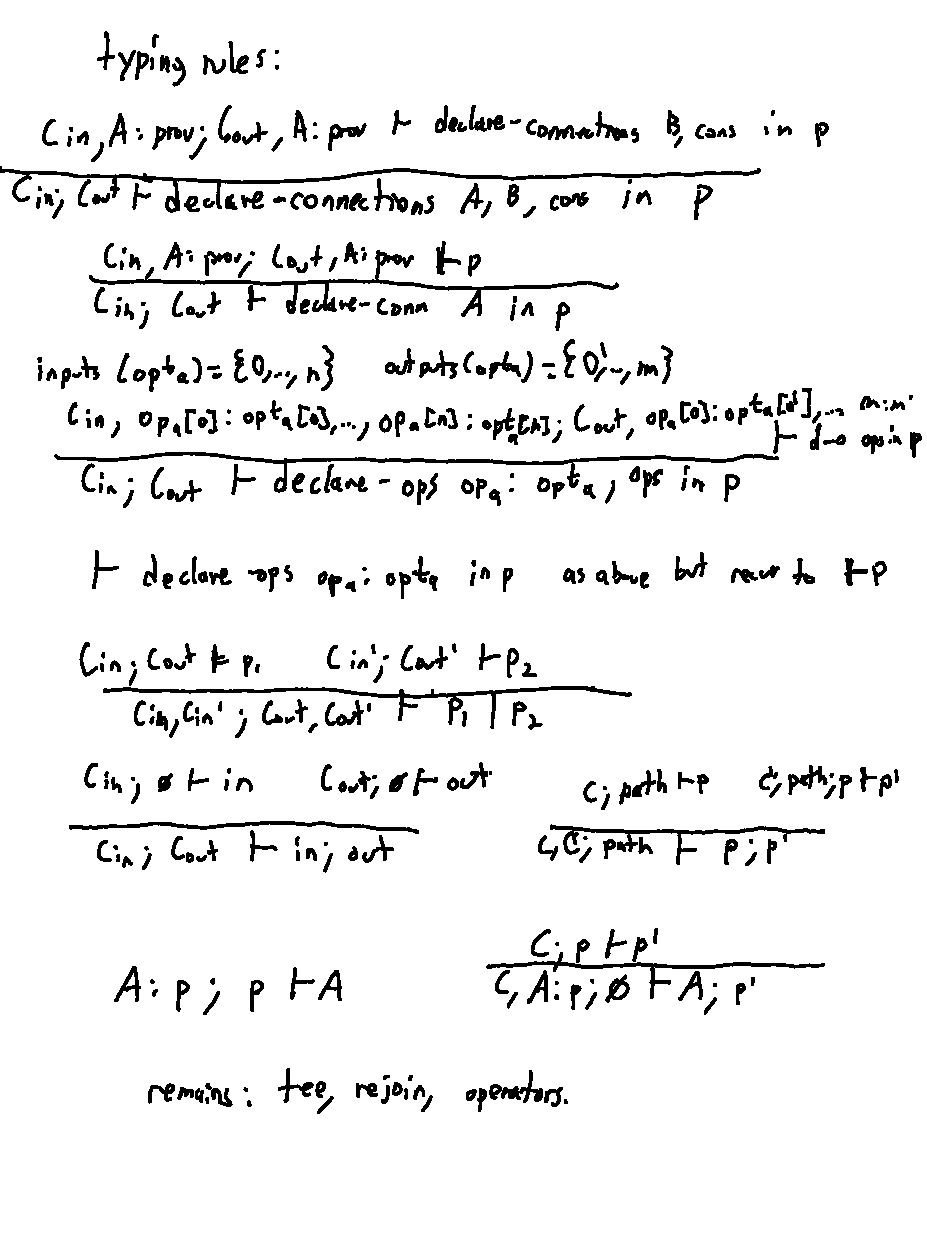
\includegraphics{freehand-types}
  \label{fig:types}
  \caption{Types: top-level}
\end{figure}
\begin{figure}
\begin{mathpar}

    {\inferrule[derivation-type-base]{}{Γ ⊢ d : τ}}

\end{mathpar}    
    \caption{Types: derivations }
    \label{fig:types2}
\end{figure}

\begin{figure}
\begin{mathpar}

{\inferrule[axoim-transform-base]{}{Γ ⊢ d ⇝ d'}}

\end{mathpar}    
    \caption{Types: axiom transformations }
    \label{fig:types3}
\end{figure}

\begin{figure}
\begin{mathpar}

    {\inferrule[exchange-C-in]
      {C,C_2,C_1,C' ;Γ ⊢ p : d~τ}
      {C,C_1,C_2,C' ;Γ ⊢ p : d~τ}}

    {\inferrule[exchange-gamma-in]
      {C ;Γ,Γ_1,Γ_2,Γ' ⊢ p : d~τ}
      {C ;Γ,Γ_2,Γ_1,Γ' ⊢ p : d~τ}}

    {\inferrule[weaken-gamma-in]
      {C ;Γ,Γ'  ⊢ p : d~τ}
      {C ;Γ,Γ_w,Γ' ⊢ p : d~τ}}

    {\inferrule[contract-gamma-in]
      {C ;Γ,Γ_c,Γ_c,Γ' ⊢ p : d~τ}
      {C ;Γ,Γ_c,Γ' ⊢ p : d~τ}}

    {\inferrule[exchange-C-out]
      {C,C_2,C_1,C' ;Γ; d ⊢ p}
      {C,C_1,C_2,C' ;Γ; d ⊢ p}}

    {\inferrule[exchange-gamma-out]
      {C ;Γ,Γ_1,Γ_2,Γ'; d ⊢ p}
      {C ;Γ,Γ_2,Γ_1,Γ'; d ⊢ p}}

    {\inferrule[weaken-gamma-out]
      {C ;Γ,Γ'; d  ⊢ p}
      {C ;Γ,Γ_w,Γ'; d ⊢ p}}

    {\inferrule[contract-gamma-out]
      {C ;Γ,Γ_c,Γ_c,Γ'; d ⊢ p}
      {C ;Γ,Γ_c,Γ'; d ⊢ p}}

\end{mathpar}    
    \caption{Types: boring structural stuff }
    \label{fig:types-structural}
\end{figure}



Worth wondering if we're going to be in trouble overloading the $[]$ syntax here; time will tell. 
Types appear in figure \ref{fig:types}. 
Another concern is that we have a uhhh _lot_ of type systems in the mix at this point: 
we've got $C;Γ;d ⊢ p : τ$, $Γ ⊢ d : τ$, and $Γ ⊢ d ⇝ d'$.  
That's a lot more independent systems than we'd ideally  have.  Is there a way to collapse this back down? 

Another important note! I think fold/unfold are wrong and unfit for purpose, actually.  We should really be replacing the variable names with their derivation expression when they're placed into the derivation context for the first time.  But as of right now, that's not how the type system works.  Maybe we need to "output" a derivation, rather than put it in the context.  Note: doing this naively immediately breaks on the dispatch to relevant-parallel and general-parallel.  I think it still holds significant promise, but might not be viable for 11:40pm.

Another note: the "natural" way to do derivations might change between a push-oriented and a pull-oriented worldview---worth thinking about / playing around with.

On the above: turns out I did stay up and push it through and... it seems to work! Shockingly! Quite Interesting. 

\section{general notes}

Something we originally wanted to do was relaxations---operators that happened to consume input $'s$, but could just as well accept any $"permute"('s)$.  How do we want to model this relaxation now, and is it still in scope? Concretely, I believe that this _is_ still in scope, and takes the form of setting translation-preservation targets to literal expressions like $"permute"('s)$.  The challenge here will be reasoning in the algebra; we're not talking about equational rewriting anymore, since we also need to include weakening ("permute" generalizes lots of transformations). 


\end{document}
